\ifpdf
	\graphicspath{{3/pic/PNG/}{3/pic/PDF/}{3/pic/}}
\else
	\graphicspath{{3/pic/EPS/}{3/pic/}}
\fi

\chapter{Numerical methods for neutron transport}\label{chap:nte-methods}

As mentioned in the introductory chapter, we will focus on deterministic methods for solving the NTE, requiring proper
discretization of \eqref{eq1} and solution of the resulting system of algebraic equations. 
In the following sections, we review some of the most widely used (in author's opinion) semi-discretizations with respect to
energy, angle and spatial variables and finish this chapter with a general discussion on solving large sparse systems of
algebraic equations, resulting from the combination of semi-discretizations that are most suitable for our purposes. We
will focus on the fixed-source problem, whose solution is a neccessary part in practically all numerical methods for
solving the generalized eigenvalue problem \eqref{eq:critical}.

\section{Approximation of energetic dependence}\label{sec:MG}

The continuous dependence on energy, $\psi = \psi(\cdot, E)$, is typically resolved by the so called \textit{multigroup
approximation}. In this approximation, the interval of neutron energies is divided as follows\footnote{Note that the
energy intervals (groups) are numbered in a descending order, i.e. a group with larger index contains lower energies than a group with
lesser index.}:
$$
\begin{multlined}
  \bigl[\Emin,\Emax] = \bigl[E^{G}-\dEh{G},E^{G}+\dEh{G}\bigr]\cup \ldots\\
  \ldots \cup \bigl[E^{g}-\dEh{g}, E^{g}+\dEh{g}\bigr] \cup \ldots \cup
  \bigl[E^1-\dEh{1},E^{1}+\dEh{1}\bigr],
\end{multlined} 
$$
and equations \eqrefs{eq1}{eq:nte3} are integrated over each energy group range 
\linebreak
\mbox{$\bigl[E^{g}-\dEh{g}, E^{g}+\dEh{g}\bigr]$}.
The NTE \eqref{eq1} is thus transformed into a finite system of integro-differential
equations, each governing the flux of neutrons with energies within a particular range (in this context called
\textit{group}):
\begin{equation}\label{eq:psi-MG}
\begin{multlined}
  \psi^g(\br, \bomega) = \frac{1}{\Delta E^{g}}\int_{g}\psi(\br, \bomega, E),\d{E} \equiv
  \frac{1}{\Delta E^{g}}\int_{E^g-\Delta E^{g}/2}^{E^g+\Delta E^{g}/2}\psi(\br, \bomega, E),\d{E},\\ g = 1, 2,\ldots
  G.
\end{multlined}
\end{equation} 
This conventional procedure leads to the following set of $G$ coupled neutron transport equations
\begin{equation}\label{eq:mg}
	\left\{
	  \begin{aligned}
      &T_G\{\psi^g(\br,\bomega)\} = \{q^g(\br,\bomega)\},\\
      &\Dom{T_G} = \bigl\{\{\psi^g\}\in \bigl[\Hp[1](X)\bigr]^G,\ \psi^g\vert_{\pX[-]} = 0,\ g = 1,\ldots,G\bigr\},
    \end{aligned}
  \right.\\[.2em]
\end{equation}
where the sets of variables with $G$ elements are understood: $\{f^g\} \equiv \{f^g\}_{g=1}^G$. The multigroup transport
operator has the following form:
\begin{equation*}
\begin{gathered}
    T_G\{\psi^g(\br,\bomega)\} = \left\{\left(A + \Sigma_r^g\right)\psi^g(\br,\bomega) - \summ{g'=1,g'\neq g}{G}
    K^{gg'}\psi^{g'}(\br,\bomega)\right\},\\
    \Sigma_r^g = \sigma_t^g(\br) - \intA[']{\kappa^{g\sla g}(\br,\bomega\cdot\bomega')},\quad K^{gg'} = 
    \intA[']{\kappa^{g\sla g'}(\br,\bomega\cdot\bomega')}
\end{gathered}
\end{equation*}
where the terms with superscript $g$ or $g'$ represent quantities suitably averaged over 
\mbox{$\bigl[E^{g}-\dEh{g}, E^{g}+\dEh{g}\bigr]$}, e.g. $K^{gg'}$ is (in theory) obtained as
\begin{equation}\label{eq:mg-kappa}
	\kappa^{gg'}(\br,\bomega\cdot\bomega') = \frac{\int_{g}\int_{g'} \kappa(\br,\bomega\cdot\bomega',E \sla
	E')\psi(\br,\bomega,E')\,\d{E'}\d{E}}{\int_{g}\psi(\br, \bomega, E)\,\d{E}}.
\end{equation}
It is customary to move the \textit{self-scattering} (diagonal) part of the
collision operator to the reaction operator. Since the reactions in which energetic distribution of both the incoming 
and outgoing neutrons lies within the same group are included in both $\sigma_t$ and $\kappa$  (compare equations
\eqref{eq:ddifxs} and \eqref{eq:st}), this transformation makes $\Sigma_r^g\psi^g$ represent the actual rate of neutron
removal from the group, while $K^{gg'}\psi^{g'}$ the rate of neutron addition to that group. Results about unique
solvability presented in previous chapter carry over to the multigroup setting by considering a counting measure on the
set $\{E^G,\ldots,E^1\}$ instead of the continuous Lebesgue measure $\d{E}$ \cite[Chap. XXI \S 2]{DautrayLions}.

Although the multigroup system of neutron transport equations has a relatively simple form, finding an optimal grouping
of energies and determining the associated group-averaged coefficients is not an easy task in most practical
applications because of the highly complicated energetic dependence of nuclear processes, as illustrated by the
typical dependence of the (microscopic) fission cross-section of \isotope[235][92]{U} in the so-called resonance range
of energies and corresponding multigroup approximation in Fig. \ref{fig:xs}.
\begin{figure}[htp]
\begin{center}
  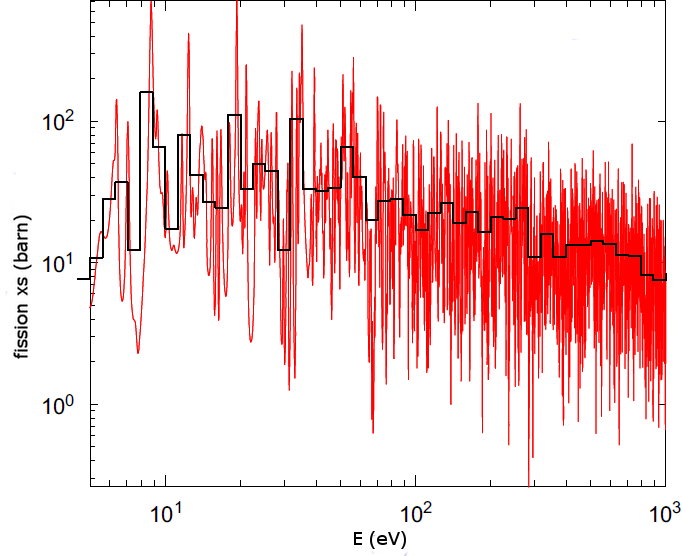
\includegraphics[scale=.4]{U235fg}
  \caption{Microscopic fission cross-section of U235}
  \label{fig:xs}
\end{center}
\end{figure}
Suitable approximation of the unknown exact solution in \eqref{eq:mg-kappa} is also highly non-trivial, albeit essential
for the success of the multigroup method. Even though an alternative to the finite-volume like approximation
\eqref{eq:psi-MG} has been proposed recently  in \cite{Douglass} -- using Galerkin projection of angular flux onto a
space of functions supported over subregions of the energy range (a finite-element like approach) --  the multigroup approximation still remains the most universally used approach to simplify the energetic dependence (see, e.g., \cite[Chap.~5]{Cacuci1} or \cite{Cho1}). However, we will
not specifically address this issue and always assume that the multigroup coefficients appearing in the equations 
are given as input.
\begin{remark}{\textsc{Fission spectrum}}
In criticality problems, the set of multigroup data must include both parts of the collision kernel
$\kappa^{gg'}$, i.e. the cross-sections $\sigma_s^{gg'}$ and $\sigma_f^{gg'}$, as well as $\nu^{g'}$ and
$\chi^g$ (neutron yield from inelastic scattering, $\eta$, is usually absorbed into $\sigma_s$). Because of the rapid
decay of $\chi(E)$ for low energies (as neutrons are mostly emitted with high energies from fission) that are
nevertheless the most important for the cross-sections (as most interactions are likely to occur due to slowly moving
neutrons, at least in classical moderated reactors)\footnote{cf. \fref{fig:xs} and \fref{fig:spectrum} and notice the
different scaling on the horizontal axis}, there will typically be $\chi^g = 0$ for $g = G,G-1,\ldots,G-k$. The
group-discretized operator $F$ from \eqref{eq:FScrit} will therefore have a non-trivial null-space, leading ultimately
to a fully discrete generalized eigenproblem of type $\mat{A}\mat{x} = \lambda\mat{B}\mat{x}$ with singular $\mat{B}$.
\end{remark}

A standard way of iterative solution of the multigroup system is the \textit{source iteration}:
\begin{equation}\label{eq:MGGS}
	\left(A + \Sigma_r^g\right)\psi^g_{(i+1)} = \summ{g'\leq g-1}{} K^{gg'}\psi^{g'}_{(i+1)} + \summ{g' \geq g+1}{}
  K^{gg'}\psi^{g'}_{(i)} + q^g,\quad g = 1,\ldots,G,\ \ i = 0,1,\ldots
\end{equation}
  This is a Gauss-Seidel iteration for the operator equation \eqref{eq:mg}, where the matrix operator $T_G$ has been
split into its lower-triangular part $A + \Sigma_r^g - K^{gg'}$ ($g'\leq g$) and its upper triangular part $K^{gg'}$
($g'> g$) and the lower triangular part is being inverted by forward substitution.
Note that a mono-energetic transport problem in group $g$ has to be solved in each iteration, and if neutron advection
can be approximated by a symmetric operator $\tilde A$, the problem would become symmetric with implications for
efficient numerical solution (see sections \ref{sec:second-order} and \ref{sec:algebraic} below). Convergence of this 
scheme can become slow when the upper triangular part (representing neutron up-scattering from lower energies to 
higher energies) is dominating. Therefore, when preparing the multigroup data, it may be advantageous to put an effort
into finding such an energy grouping that minimizes the up-scattering.
\begin{remark}\label{rem:SI}
Here we assume that the
mono-energetic problem can be solved exactly. Some transport approximations (like the $\SN$ method presented in
\sref{sec:1-SN}) typically employ another iteration level to resolve angular coupling of the within-group fluxes
induced by scattering. This iteration can also become very slow if scattering of
neutrons with given energy dominates their absorption and some acceleration is usually needed (we will return to this
issue later in \sref{sec:SI}).
\end{remark}

In the remainder
of this chapter, we will focus on the approximation of neutron flux in a single
group (index of which will be omitted), described by the corresponding within-group equation in which contributions from
other groups are encapsulated in the source term $\src$.

\section{Approximation of angular dependence}

A big number of methods have been proposed for approximating the angular dependence of neutron
flux. Many of them are still used and actively developed today as their characteristics make them more suitable for one
application area than other methods, which are preferred in different areas.

\subsection{Lattice calculations} \label{sec:lattice}
As a first example, we consider the class of
methods originally derived from the equivalent integral form of the NTE (see \sref{sec:advection}). Typical
representatives of this class are the method of collision probabilities or the method of characteristics (see e.g.
\cite{Cho2,Wu1,Hursin1,Petkov1,Sanchez1}). As the integral form of the NTE represents the global neutron balance over
the domain, the corresponding algebraic systems (obtained after spatial discretization) are full and
their solution demanding on computer resources. On the other hand, these methods quite naturally handle complex
geometries. Taking into consideration smaller geometric features of the domain, we are effectively coming from a
macroscopic scale to a mesoscopic range where the neutrons direction of motion as well as their kinetic energy become
more significant. High degree of spatial coupling and the requirement of fine resolution of angular and energetic
dependence does not make these methods suitable for whole-core reactor calculations.
However, these small-scale,
high-fidelity calculations\footnote{called \textit{lattice calculations} as they are typically performed on a single
representative subdomain of the core (one or several neighboring assemblies of fuel pins, or the fuel pin itself)
with reflective boundary conditions, simulating an infinite lattice of such subdomains} are indispensable for
generating appropriately averaged coefficients for the computationally more feasible larger scale calculations.
This \textit{spatial homogenization} and \textit{energy group condensation} (already mentioned in the previous
section), as these averaging procedures are traditionally called in nuclear engineering field, are employed by many existing whole-core simulators (see e.g.
\cite[Chap. 17]{Reuss1} or the review in first two sections of \cite{Sanchez7}). To simulate a long-term nuclear reactor
operation, it is furthermore neccessary to perform these procedures under varying physical conditions of the core and
generate many sets of averaged coefficients corresponding to these conditions. The code system described in
\cref{chap:coupled} expects these coefficient sets on input, i.e., it is not designed for lattice calculations.

\vspace*{1em}
More suitable for whole-core calculations are methods derived from the integro-differential
version of the NTE, eq.
\eqref{eq1}, which lead to sparse algebraic systems. The most successful and well-established are the method
of discrete ordinates ($\SN$) and the method of spherical harmonics ($\PN$).
Both arise from applying in the
angular domain a classical well known approach for constructing finite numerical
approximations of PDEs. Although in the final code, we ultimately use the lowest order approximation that can be obtained
equivalently from both approaches (the neutron diffusion model) we will briefly introduce the main ideas behind the
$\SN$ and $\PN$ methods and expose their most important properties in the next two subsections. These properties are
generally known, but their origin in mathematical structure of the equations is mostly overlooked in
literature (rare exceptions will be cited below and in the corresponding appendices). 

\subsection{The $\SN$ method}\label{sec:1-SN}
The basic $\SN$ method uses the collocation approach in which a set of directions (\textit{ordinates})
$\omega = \{\bomega_n\}_{n=1}^{M}$ is chosen and the solution is approximated as:
\begin{equation}\label{eq:sn_approx} 
	\psi(\br, \bomega) \approx 
		\pw{\psi(\br,\bomega_n)}{if $\bomega = \bomega_n$ for $\bomega_n \in \omega$}
		   {0}{if $\bomega \not \in \omega$.} 
\end{equation}
Equation \eqref{eq1} as well as the boundary conditions \eqref{eq:nte2} or \eqref{eq:nte3} are then evaluated at these
$M = M(N)$ isolated directions. Notice that reflective (or albedo) boundary conditions place restrictions on the set of
ordinates as it should optimally contain both directions of each reflected pair (otherwise an interpolation would be
needed). For the traditional direction sets, we have $M = N(N+2)$ if the given problem does not possess any symmetries;
the method of discrete ordinates using such a number of directions is traditionally refered to as the method of 
discrete ordinates of order $N$, shortly $\SN$.

To evaluate the integral term on the right hand side of the equation, the set of directions is accompanied by a
corresponding set of weights $\{w_n\}_{n=1}^{M}$, together defining a quadrature of the sphere $\Sphere$. The
requirement of accurate evaluation of the integral term of eq.
\eqref{eq1} as well as accurate integration of the angular flux function over the sphere (to obtain the scalar flux)
constitutes the main guideline for the choice of directions and weights. We will return to this matter later in 
\sref{sec:DO}; for now it suffices to say that for three-dimensional problems without any symmetries, \mbox{$M = \left|\{\bomega_n, w_n\}\right| = \Oh(N^2)$} (with the
value of $M$ for typically used quadrature sets stated above).

To write  the final result of the $\SN$ approximation, let us first denote for a set $s = \{c_k\}_{k=1}^n$ the column
vector with entries $c_1,c_2,\ldots,c_n$ as $\col s$ and similarly the diagonal matrix whose diagonal is
given by elements of $s$ as $\diag(s)$. Then, denoting
\begin{equation}\label{eq:sn_vecs}
\psi_n(\br) \equiv \psi(\br,\bomega_n), \quad q_n(\br) \equiv
q(\br,\bomega_n),\quad n = 1,\ldots, M	
\end{equation}
we will define the vector of angular fluxes and the vector angular sources as
\begin{equation}\label{eq:sn_vars}
\Psi(\br) := \col\{\psi_n(\br)\}_{\idxset{M}},\quad
\mat{Q}_{S_N}(\br) := \col\{q_n(\br)\}_{\idxset{M}},
\end{equation}
where we used the index set of $\SN$ variables: $\idxset{M} = \{1,2,\ldots,M\}$.
The $\SN$ approximation consists of the following set of $M$ PDEs in spatial domain\footnote{Differentiation and
integration of vector functions (such as the term $\pd{\Psi(\br)}{x}$ in eq. \eqref{eq:sn1}) is conventionally
understood component-wise.}:
\begin{equation}\label{eq:sn1} 
\mat{A}_{S_N}^x\pd{\Psi(\br)}{x} + \mat{A}_{S_N}^y\pd{\Psi(\br)}{y} +
\mat{A}_{S_N}^z\pd{\Psi(\br)}{z} + \bigl[\sigma_t(\br)\mat{I} - \mat{K}_{S_N}(\br)\bigr]\Psi(\br) = \mat{Q}_{S_N}(\br),
\end{equation}
where $\mat{I}$ is the $M\times M$ identity matrix and
$$
	\mat{A}_{S_N}^x = \diag\{\Omega_{n,x}\}_{\idxset{M}},\ \mat{A}_{S_N}^y = \diag\{\Omega_{n,y}\}_{\idxset{M}},\
	\mat{A}_{S_N}^z = \diag\{\Omega_{n,z}\}_{\idxset{M}}.
$$

\subsubsection{Structure of the $\SN$ approximation}
Equation \eqref{eq:sn1} represents a system of advection-reaction equations, each with constant advection field given by
the matrices $\mat{A}_{S_N}^x, \mat{A}_{S_N}^y, \mat{A}_{S_N}^z$.  The system is coupled through the term
$
	\mat{K}_{S_N}\Psi,
$
whose $m$-th component ($1 \leq m \leq M$) is given by
$$
\sum_{n=1}^{M} w_n \kappa(\bomega_m\cdot\bomega_n) \psi_n,\quad \bomega_n,\bomega_m\in \omega,\ 
	w_n\in \mathcal{W}
$$
We can therefore see full unknown coupling. In order to recover sparsity (and also facilitate the use of efficient
constant-advection solvers based on explicit marching in the advection direction), the so-called  \textit{scattering
source iteration} is utilized, in which the system \eqref{eq:sn1} is fully decoupled by moving $\mat{K}_{S_N}$ to the
right. Each equation is solved separately using any method suitable for an advection-reaction PDE with constant
advection vector, using $\psi_n$ from previous iteration to evaluate $\mat{K}_{S_N}\Psi$. Classical iteration methods
like Jacobi and Gauss-Seidel are typically used to update $\Psi$ during the iteration process; e.g. the Jacobi scheme 
gives the iteration
\begin{equation}\label{eq:SI}
	\mat{A}_{S_N}^x\pd{\Psi_{(i+1)}}{x} + \mat{A}_{S_N}^y\pd{\Psi_{(i+1)}}{y} +
	\mat{A}_{S_N}^z\pd{\Psi_{(i+1)}}{z} + \sigma_t\mat{I}\Psi_{(i+1)}= \mat{K}_{S_N}\Psi_{(i)} +
	\mat{Q}_{S_N},\quad
	i = 0,1,\ldots
\end{equation}
for given initial approximation $\Psi_{(0)}$. We will return to the convergence characteristics of this iteration later;
for now, assume that a converged solution vector $\Psi = \colset{\psi_n}{M}$ has been obtained. The important physical
quantities (scalar flux, neutron current) are then obtained directly from their definition \eqref{eq:scalar_flux} and \eqref{eq:bJ} using
the quadrature formula, e.g.
$$
	\phi(\br) = \intA{\psi(\br,\bomega)} = \sum_{n=1}^{M} w_n \psi(\br,\bomega_n) = \sum_{n=1}^{M} w_n \psi_n, \quad \br\in
	\VV,\ \bomega_n\in \omega,\ w_n\in \mathcal{W}.
$$

\myparagraph{Ray effects}
A major drawback of the $\SN$ angular approximation comes from the fact that it propagates radiation 
only in a discrete set of directions. Only in the limiting case of infinite number of directions will the
whole phase space be covered. Otherwise, there will remain under-treated regions, while other regions will receive more radiation in order
to satisfy the global balance. This will lead to spatial oscillations of the scalar flux  known as the \textit{ray
effects}. The root cause of ray effects is often attributed to the intuitively obvious lack of rotational invariance 
(\cite{Reuss}, \cite{Sanchez6}), which shows that the important property of the NTE is not carried over to the $\SN$
approximation. Various remediesWe give now a rigorous proof of this fact for the simplified transport problem without
scattering, using the operator form of the $\SN$ equations developed in the previous subsection. We remark that scattering can somewhat ameliorate the
 oscillations caused by ray effects as it increases the coupling between directional fluxes, but it cannot remove the
 inherent lack of rotational invariance of the $\SN$ approximation.

\subsubsection{Operator form}\label{sec:opsn}
In order to exhibit differences between the $\SN$ approximation and the $\PN$ approximation presented in the following
section, we write both methods as projections onto an appropriate approximation subspace. To continue our functional
analytic  We will see that the $\SN$ approximation space is quite poor and solutions found in this subspace by solving
the $\SN$ system do not possess important properties of the true solution of the NTE, like the rotational invariance. 

First, note that the $\SN$ approximation concerns only the angular variable. To reduce clutter, we will therefore drop
the spatial variable in the following discussion.
Consider now an arbitrary $\SN$ approximation specified by the given set of ordinates
$\omega = \{\bomega_n\}_{\idxset{M}}$ and a corresponding set of quadrature weights $\mathcal{W} =
\{w_n\}_{\idxset{M}}$.
%by using the Dirac measure $\delta_{\bomega}(\bomega')$ with the property
%\begin{equation}\label{eq:dirac}
%	\int_{\Sphere} f(\bomega')\d{\delta_{\bomega}(\bomega')} = f(\bomega).
%\end{equation}
For a vector (of functions of spatial variable) $\mat{F} = \colset{f_n}{\idxset{M}}$, we define the mapping
\begin{equation}\label{eq:map_SN}
\begin{gathered}
\PiSN: \mat{F} \mapsto f\in V_{S_N},\\
\bigl(\PiSN \Psi\bigr)(\bomega) = 
\pw{\psi_n}{if $\bomega = \bomega_n$ for $\bomega_n \in \omega$}{0}{if $\bomega \not
	\in \omega$}
\end{gathered}
\end{equation}
$V$ is some general function space ensuring existence of unique solution of the NTE (see \sref{sec:fixed-source} for
examples) and $V_{S_N}\subset V$ is its subspace containing functions vanishing (as functions of $\bomega$) everywhere
on $\Sphere$ except at $\bomega \in \omega$. Note that this mapping converts a vector of directional fluxes to a 
function on $\Sphere$. Corresponding to it is the mapping that produces the discrete ordinates representation of a 
function $f$ defined on $\Sphere$:
\begin{equation}\label{eq:map_SN_inv}
	\PihSN f(\bomega) := \col\left\{f_n \right\}_{\idxset{M}}
	 = \col\left\{f(\bomega_n)\right\}_{\idxset{M}}
\end{equation}
(which we implicitely used in \eqref{eq:sn_vars} with $f(\cdot,\bomega) = \psi(\cdot,\bomega)$ and
$f(\cdot,\bomega) = q(\cdot,\bomega)$, respectively, and which also applies to functions representing the
inflow boundary conditions).
With these two mappings, we can rewrite the $\SN$ system \eqref{eq:sn1} in terms of the transport operators from eq.
\eqref{eq1op}:
\begin{equation}\label{eq:sn_op}
	\PihSN (\op{L} - \op{K}_{S_N}) \PiSN \Psi = \mat{Q}_{S_N},
\end{equation}
where $\op{K}_{S_N}: V_{S_N} \to V$ is the $\SN$ quadrature representation of the original integral operator
$K$, defined as follows: 
\begin{equation}\label{eq:KSN}
	\op{K}_{S_N} f(\bomega) = \sum_{n=1}^{M} w_n \kappa(\bomega\cdot\bomega_n) f(\bomega_n), \quad \bomega_n\in \omega,\ 
	w_n\in \mathcal{W}. 
\end{equation}
Note that the operator $\PihSN (\op{L} -
\op{K}_{S_N}) \PiSN$ maps $M$-vectors to $M$-vectors and represents the $\SN$ matrix. The
final $\SN$ approximation of the original transport operator is obtained as an operator $V \to V_{S_N}$ by incorporating the definition of the $\SN$ unknowns $\Psi$ from a function
$\psi \in V$ and representing the output again as a function. This leads to the following formulation:
\begin{equation}\label{eq:sn_op}
	\PiSN \PihSN (\op{L} - \op{K}_{S_N})\PiSN \PihSN \psi = \PiSN \PihSN q,
\end{equation}
or
\begin{equation}\label{eq:sn_op2}
	\Projop[S_N]  (\op{L} - \op{K}_{S_N}) \Projop[S_N] \psi = \Projop[S_N] q
\end{equation}
where
\begin{equation}\label{eq:proj_sn}
	\Projop[S_N] := \PiSN \PihSN, \quad \Projop[S_N] : V \to V_{S_N}.
\end{equation} 
It is clear from the definitions \eqref{eq:map_SN} and \eqref{eq:map_SN_inv} that when restricted to $V_{S_N}$, 
\linebreak[3]\mbox{$\PihSN = \PiSN^{-1}$} and hence $\Projop[S_N]^2 = Id$, where $Id : V_{S_N} \to V_{S_N}$ is the
identity operator on $V_{S_N}$.
 Therefore, $\Projop[S_N]$ represents a projection onto the $S_N$ approximation space (and formalizes eq.
 \eqref{eq:sn_approx}).


\label{sec:SI}
\comment{
Writing the iteration in the form
$$
\PihSN \op{L} \PiSN  \Psi_{(i+1)} = \PihSN \op{K}_{S_N} \PiSN \Psi_{(i)} + \mat{Q}_{S_N},
$$
we can see that propert It can be shown by Fourier analysis that
in an infinite homogeneous medium, the iteration \eqref{eq:SI} suppresses those Fourier modes with wavelengths  see also Remark \ref{rem:SI}).
\cite[Chap. 1]{Azmy1}, or \cite[Sec. II.A]{Adams})
}



 
\begin{theorem*}\label{thm:commut_NTE}
Let $L : V\to V$ be the advection-collision operator of the NTE satisfying
$RL = LR$ for all $R\in\mathrm{SO}(3)$. 
Then the corresponding $\SN$ approximation operator
\begin{equation}\label{eq:sn_op_app}
	\Projop[S_N]\op{L}\Projop[S_N]
\end{equation}
(with $\Projop[S_N]$ defined by \eqref{eq:proj_sn}, \eqref{eq:map_SN}, \eqref{eq:map_SN_inv} and particular
ordinates and quadrature sets \mbox{$\omega = \{\bomega_n\}_{\idxset{M}}$, $\mathcal{W} = \{w_n\}_{\idxset{M}}$})
satisfies $$
\op{R}\op{L}\Projop[S_N] = \op{L}\Projop[S_N]\op{R}\quad \forall R\in\mathrm{SO}(3)
$$
if and only if
\begin{equation}\label{eq:thm1_cond}
	\forall n\in \idxset{M}\ \exists m\in\idxset{M}: \mat{R}\bomega_n = \bomega_m \quad \forall \mat{R}\in\mathrm{SO}(3).
\end{equation} 
\end{theorem*}
\begin{remark*}
	Note that the conditions \eqref{eq:thm1_cond} can be satisfied only in the limit \mbox{$M\to\infty$}.
\end{remark*}
\begin{proof}
First, recall from \sref{sec:opsn} that for any $\SN$ approximate function \mbox{$f_{S_N}\in V_{S_N}$}, 
$$
	\Projop[SN]f_{S_N} = f_{S_N}.
$$
Also, for $\psi_{S_N} \in V_{S_N}$:
$$
	\bomega\cdot\nabla\psi_{S_N}(\br,\bomega) = \left.\pw{
		\bomega_n\cdot\nabla\psi(\br,\bomega_n)}{if $\bomega = \bomega_n$ for $\bomega_n\in\omega$}
		{0}{if $\bomega \not \in \omega$.}\right\} \in V_{S_N}
$$
where we recall the characterization of $V_{S_N}$ as a space of functions that, as functions of $\bomega$, vanish
everywhere on $\Sphere$ except points corresponding to the selected ordinates set. Therefore for $\psi_{S_N} \in
V_{S_N}$, 
$$
	L\psi_{S_N} \equiv \bomega\cdot\nabla\psi_{S_N} + \sigma_t\psi_{S_N} \in V_{S_N}.
$$
Since \mbox{$\Rng (\PiSN) = V_{S_N}$}, it follows that the $\SN$ operator \eqref{eq:sn_op_app} can be simplified as:
\begin{equation}\label{eq:sn_op2}
	\Projop[S_N]\op{L}\Projop[S_N] = \op{L} \Projop[SN].
\end{equation}
Because of the commutativity of $L$ and $R$, it therefore suffices to show that $\Projop[S_N]$ commutes
with $\op{R}$, that is (using def. \eqref{eq:proj_sn})
\begin{equation}\label{eq:thm1_point}
	R \PiSN \PihSN \psi = \PiSN \PihSN R \psi\quad  \forall \psi \in V, 
\end{equation}
if and only if the condition \eqref{eq:thm1_cond} holds.\\[.2em] 

As in \sref{sec:opsn}, we will suppress the spatial dependence as the $\SN$ approximation concerns only the angular
dependence. For any $\psi\in V$, we have
\begin{equation*}
	\PihSN R\psi(\bomega) = \colset{R\psi(\bomega_n)}{\idxset{M}} = \colset{\psi(\mat{R}^T\bomega_n)}{\idxset{M}}.
\end{equation*}
Applying $\PiSN$ thus yields a function $f_\psi = \PiSN\PihSN R\psi \in V_{S_N}$ such that
\begin{equation}\label{eq:thm1_f}
f_\psi(\bomega) = \pw{\psi(\mat{R}^T\bomega_n)}{if $\bomega = \bomega_n$ for $\bomega_n\in\omega$}{0}{if $\bomega \not
	\in \omega$.}
\end{equation}
On the other hand, let $u = \PiSN\PihSN\psi$. Then
$$
u(\bomega) = \pw{\psi(\bomega_n)}{if $\bomega = \bomega_n$ for $\bomega_n\in\omega$}{0}{if $\bomega \not
	\in \omega$}
$$ 
and the rotated function $g_\psi(\bomega) = R\PiSN\PihSN\psi = R u(\bomega)$ is given by
$$
g_\psi(\bomega) = u(\mat{R}^T\bomega) = \pw{\psi(\bomega_n)}{if $\mat{R}^T\bomega = \bomega_n$ for
$\bomega_n\in\omega$}{0}{if $\mat{R}^T\bomega \not \in \omega$}
$$
or, equivalently, by
\begin{equation}\label{eq:thm1_g}
g_\psi(\bomega) = \pw{\psi(\bomega_n)}{if $\bomega = \mat{R}\bomega_n$ for
$\bomega_n\in\omega$}{0}{if $\bomega \not \in \mat{R}\omega$}
\end{equation}
(where action of $\mat{R}$ on the set $\omega$ is understood element-wise). If the ordinate set $\omega$ contains for
any ordinate $\bomega_n$ also its rotated copy $\mat{R}\bomega_n$, i.e., condition \eqref{eq:thm1_cond} holds, then also
$$
	\bomega_n = \mat{R}^T\bomega_m
$$
and after simple substitution in \eqref{eq:thm1_g} and renumbering in \eqref{eq:thm1_f}, we obtain
$$
	f_\psi(\bomega) = g_\psi(\bomega).
$$
In order for this equality to hold true for any $\psi \in V$ (and hence for \eqref{eq:thm1_point} to hold true), the
condition \eqref{eq:thm1_f} is also necessary.
\end{proof}


\subsection{The $\PN$ method}\label{sec:PN}

Instead of the collocation method used by the $\SN$ approximation, the $\PN$ method uses the Galerkin weighted residuals
approach in the angular domain. That is, the angularly dependent quantities in \eqref{eq1} are expanded into infinite
series of properly chosen functions that span a complete basis on the unit sphere, the equation is multiplied by each member of the basis in turn
and integrated over the sphere. The properties of the basis functions are then used to derive equations for
the expansion coefficients. Only a finite number of the expansion terms is considered to allow practical computation.
Usually, the expansion is truncated to a finite length of $K = K(N)$ terms\footnote{The length of the expansion $K$
should not be confused with the operator $K$ introduced in the previous section; it will be always clear from context 
which meaning the letter $K$ currently has.} by setting all expansion coefficients with higher index to 0 (although there exist alternative closure methods that may have favorable properties in certain situations, see e.g.
\cite{Frank0}). Then we speak of the $\PN$ approximation:
\begin{equation}\label{eq1.1}
  \psi(\br,\bomega) \approx \sum_{k=1}^{ K} \phi_k(\br) f_k(\bomega).
\end{equation}
A natural function space to support this procedure is the Hilbert space of 
square-integrable functions on the sphere $\Lp[2](\Sphere)$, equipped with the inner product
\begin{equation}\label{eq:s2_ip}
	(u, v)_{\Lp[2](\Sphere)} = \intA{u(\bomega) {v(\bomega)}}.
\end{equation}
We will therefore assume \mbox{$\psi(\cdot,\bomega)\in\Lp[2](\Sphere)$} in this section. 

The system of spherical basis functions that were used in the original $\PN$ method are the
\textit{spherical harmonic functions} (shortly \textit{spherical harmonics}, App. \ref{app:SH}). We will consider
here the real system (whose elements are sometimes called \textit{tesseral spherical harmoncs}) as it is more convenient
for practical purposes than the equivalent complex system (which appears to be more traditional in nuclear engineering 
literature, e.g. \cite[Sec. 9.7]{Stacey}, \cite[Sec. 14.4]{Reuss}), \cite[Chap. V]{Stammler}). Spherical harmonics form
a complete orthonormal system on $\Lp[2](\Sphere)$ with respect to the inner product \eqref{eq:s2_ip} (or its Hermitian 
variant when complex spherical harmonics are used) and simplify the algebraic manipulations needed to arrive at the 
conditions for coefficients $\phi_k$ (called \textit{angular moments}). In one dimension, spherical harmonics reduce to 
Legendre polynomials and $ K(N) = N$.
For general three-dimensional problems, there are $2n + 1$ linearly independent spherical harmonics for each degree $n$ 
and 
$$ 
	K(N) = \sum_{n=0}^{N} 2n + 1 = (N+1)^2.
$$

The approximation \eqref{eq1.1} is usually rewritten as
\begin{equation}\label{eq:pn_approx}
	\psi(\br,\bomega) \approx \sum_{k=1}^{ K} \phi_k(\br)\Y{k}{}(\bomega) \equiv
	\suma[n]{0}{N}\suma[m]{-n}{n}\angmom{n}{m}(\br)\Y{n}{m}(\bomega)
\end{equation}
where $\Y{n}{m}(\bomega)$ is the spherical harmonic function of degree $n$ and order $m$
and in the first term on right, we consider the single index $k$ ($1 \leq k \leq  K$) that covers all the combinations of $n$ and $m$ ($0 \leq n \leq N$, $-n\leq m \leq n$) appearing in the second term. We finally arrive at a system of $ K$
partial differential equations in spatial domain which is of comparable size as the system of $\SN$ equations and has the following form:
\begin{equation}\label{eq:pn1}
	\mat{A}^x_{P_N}\,\pd{\Phi(\br)}{x} + \mat{A}^y_{P_N}\,\pd{\Phi(\br)}{y} + \mat{A}^z_{P_N}\,\pd{\Phi(\br)}{z} +
	\bigl[\sigma_t(\br)\mat{I} - \mat{K}_{P_N}(\br)\bigr]\Phi(\br) = \mat{Q}_{P_N}(\br),
\end{equation}
where 
\begin{equation}\label{eq:pn_vectors}
	\Phi = \col\left\{\phi_k\right\}_{\idxset{K}} \ \text{ and }\ 
	\mat{Q}_{P_N} = \col\left\{q_k\right\}_{\idxset{K}}
\end{equation}
are, respectively, the vector of angular flux
moments and angular source moments, and the index set of $\PN$ variables is defined analogously to the $\SN$ case:
$$
\idxset{K} = \{1,2,\ldots,K\}.
$$
The
Galerkin procedure results in their special form
\begin{equation}\label{eq:pn_angmom}
	\phi_k = (\psi, \Y{k}{})_{\Lp[2](\Sphere)},\quad q_k = (q, \Y{k}{})_{\Lp[2](\Sphere)}
\end{equation}
which, in view of \eqref{eq:pn_approx} and the completeness and orthogonality properties of spherical harmonics, also 
shows that the angular flux in the $\PN$ method is actually approximated by its orthogonal projection onto the
finite-dimensional subspace $\Lp[2]_K(\Sphere)\subset\Lp[2](\Sphere)$:
\begin{equation}\label{eq:PN_proj}
	\Projop\psi(\cdot,\bomega) := \sum_{k=1}^{ K}\ips{\psi}{\Y{k}{}} \Y{k}{}(\bomega).
\end{equation}
We also have a direct correspondence of the first four moments and the physically important quantities defined in
\sref{sec:qoi}:
$$
	\phi = \sqrt{4\pi}\angmom{0}{0},\quad \bJ = \sqrt{\frac{4\pi }{3}}\, [\angmom{1}{1}, \angmom{1}{-1}, \angmom{1}{0}]^T.
$$

\subsubsection{Operator form} \label{sec:pn_op}
As in the $\SN$ case, the $\PN$ system \eqref{eq:pn1} can be put into a form involving the transport operators from eq.
\eqref{eq1op}.
In order to do so, let us define mappings that take the vector $\Phi(\cdot)$ of angular flux moments to angular
flux $\psi(\cdot,\bomega)\in\Lp[2]_K(\Sphere)$ and vice versa. The general operators realizing this operation for the
case $\mat{F} = \Psi$ and $f(\bomega) = \psi(\cdot,\bomega)$, respectively, are
\begin{equation}\label{eq:pn_op_def}
\bigl(\PiPN\mat{F}\bigr)(\bomega) := \sum_{k=1}^{ K} f_k\Y{k}{}(\bomega), \quad
\PihPN f(\bomega) = \col \left\{(f, \Y{k}{})_{\Lp[2](\Sphere)}\right\}_{\idxset{K}}.
\end{equation} 
Using \eqref{eq:pn_angmom}, \eqref{eq:pn_vectors} and \eqref{eq:PN_proj}, we can see that 
$$
\PiPN\Phi = \PiPN\PihPN \psi = \Projop\psi.\footnote{Again as in the $\SN$ case, when restricted to the space of functions that (as functions of $\bomega$) can be
expressed as linear combination of spherical harmonics up to degree $N$, $\PihPN = \PiPN^{-1}$ (which is equivalent to $\Projop[P_N]$ being
a projection).}
$$ 
The operator form of the $\PN$ system is thus
\begin{equation}\label{eq:pn_op}
	\PihPN (L-K) \PiPN\Phi = \mat{Q}_{P_N} = \PihPN q
\end{equation}
or
\begin{equation}\label{eq:pn_op2}
	\Projop (L-K) \Projop\psi = \Projop q.
\end{equation}

\subsubsection{Structure of the $\PN$ system}
The system has the same form as that for the $\SN$ approximation, but the advection matrices:
\begin{equation}\label{eq:advmat_PN}
	\left[\mat{A}_{P_N}^s\right]_{k,l} = \intA{\Omega_s \Y{k}{}(\bomega)\Yc{l}{}(\bomega)},\quad s\in\{x,y,z\},\ 
	1 \leq k,l \leq  K
\end{equation}
are no longer diagonal (although they couple no more than 6 angular flux moments, see \ref{app:C} for an example for $N
= 3$ or \cite[App. A]{Sanchez8} for general treatment). On the other hand, the collision matrix $\mat{K}_{P_N}$ is
diagonal (as we explicitely show in App. \ref{app:C}), which makes the method computationally more attractive than the 
fully coupled $\SN$ method in cases when scattering source iteration cannot be efficiently used. However, it also
complicates the formulation of boundary (and interface) conditions. Each of the advection matrix \eqref{eq:advmat_PN} 
is symmetric and hence for any $\bn = [n_x,n_y,n_z]^T$, 
$$
	\mat{A}_{P_N}^{\bn} = n_x \mat{A}_{P_N}^x + n_y \mat{A}_{P_N}^y + n_z \mat{A}_{P_N}^z
$$
is symmetric and diagonalizable with real eigenvalues. The $\PN$ system is thus (strongly) hyperbolic in the sense of 
\cite[Def. 18.1]{leveque} (as is obviously the already diagonal system of $\SN$ equations). The eigenvalues depend on 
$\bn$ only through its length $\norm{\bn}$ (see \sref{sec:app-adv} for an example when $N = 3$,  though this property
holds for general $N$), which shows that the $\PN$ system propagates radiation at the same speed in any
direction\footnote{Here we consider the $\PN$ system as a steady-state limit of the time-dependent equation, as
explained in \sref{sec:app-adv}.}.
This hints that rotational invariance of the NTE is preserved by the $\PN$ system, as we will directly show in 
\sref{sec:dirinvPN}. The eigenstructure of the advection matrices also provides a clue on how many boundary conditions
should be prescribed for the $\PN$ system. Matrix $A_{P_N}^{\bn}$ for given $N$ has
$N(N+1)/2$ positive eigenvalues, $N(N+1)/2$ negative eigenvalues and $K(N) - N(N+1) = N+1$ zero eigenvalues,
irrespective of $\bn$. If we take $\bn$ to be the unit outward normal to $\pV$, these eigenvalues correspond,
respectively, to outgoing, incoming and tangential neutron radiation waves. In order for the hyperbolic system to be
well-posed, we are allowed to prescribe only the incoming waves, hence we are allowed to specify $N(N+1)/2$ boundary
conditions at any point of the boundary. It is more difficult to determine what the conditions actually look like as the
waves generally contain components of all moments $\angmom{n}{m}$. On the grounds of physical reasoning
(e.g. \cite{Rumyantsev}), variational analysis (e.g. \cite{Davis}) or most recently the equivalence between hyperbolic
and elliptic forms of the $\PN$ equations (\cite{Sanchez8}), the agreed upon form of $\PN$ boundary conditions
consistent with the present Galerkin framework is obtained (e.g. for the incoming condition \eqref{eq:nte2}) as:
$$
\begin{gathered}
	\left(\psi_\text{in} - \left.\Projop[P_N]\!\psi\right\vert_{\pX[-]}, \Y{p}{m} \right)_{\Lp[2](\pX[-])} = 0,\\[.35em] 
	p = 
	\left.\begin{cases}
		0,2,4,\ldots,N\!-\!1 & \mbox{ for $N$ odd}\\
		1,3,5,\ldots,N\!-\!1 & \mbox{ for $N$ even}	
	\end{cases}\right\},\ -p \leq m \leq p;
\end{gathered}
$$
that is, as (oblique) projection of the specified incoming angular flux onto $\Lp[2]_N(\pX[-])$, orthogonal
to the subspace of $\Lp[2](\pX[-])$ spanned by spherical harmonics with even/odd degrees, with respect to the inner product
$$
	\left(u,v\right)_{\Lp[2](\pX[-])} = \int_{\pV}\int_{\bomega\cdot\bn < 0}\abs{\bomega\cdot\bn}
	u(\br,\bomega)v(\br,\bomega)\,\d{\br}\d{\bomega}.
$$
We will call boundary conditions of this form (as in \cite{Davis}) \textit{Marshak boundary conditions}.


\subsubsection{Rotational invariance of the $\PN$ equations}\label{sec:dirinvPN}
The increased coupling between the unknowns in the $\PN$ system is the price for rotational invariance of spherical
harmonics that prevents ray effects appearing in $\SN$ solutions. To prove it, we will use some well known facts about
spherical harmonics (see e.g, \cite[Chap.
3]{Sansone}, \cite[Sec. 3.9]{Schreiner}). 

\myparagraph{Orthogonal decomposition of $\Lp[2](\Sphere)$}
Spherical harmonic functions of given degree $n$ generate a rotationally invariant subspace
of $\Lp[2](\Sphere)$, which we denote by $\Lambda_n$:
\begin{equation}
	\label{eq:subspace}
    	\Lambda_n = \text{Span}\bigl\{\Y{n}{m}; -n \leq m \leq n\bigr\},
\end{equation}
This means that $\op{R}(\Lambda_n) \subset \Lambda_n$ for any rotation transformation $\op{R}\in\mathrm{SO}(3)$ (cf. the
paragraph on ray effects in \Sref{sec:1-SN}). Moreover, there is no proper subspace $\Lambda_n' \subset \Lambda_n$ that
is rotationally invariant by itself. For given $n$, $\Lambda_n$ is the eigenspace associated with
the $n$-th eigenvalue of the Laplace operator on $\Sphere$:
$$
	\lap_{\Sphere} \Y{n}{m}(\bomega) = -n(n+1)\Y{n}{m}(\bomega) \quad \forall -n \leq m \leq n.
$$

Being finite-dimensional eigenspaces of a self-adjoint operator
corresponding to different eigenvalues, $\Lambda_n$ for $n=0,1,\ldots$ are mutually orthogonal, closed subspaces of
$\Lp[2](\Sphere)]$ and $\Lp[2](\Sphere) = \bigoplus_{n=0}^{\infty}\Lambda_n$\nomenclature[S]{$\bigoplus$}{direct sum of
spaces}.
Restricting to a finite direct sum, we can hence write the $\PN$ projection \eqref{eq:PN_proj} as
\begin{equation}\label{eq:pn_approx2}
	\Projop\psi(\cdot,\bomega) = \suma[n]{0}{N}\Projop[\Lambda_n]\psi(\cdot,\bomega),
\end{equation}
where 
$$
	\Projop[\Lambda_n]\psi(\br,\bomega) = \suma[m]{-n}{n}\angmom{n}{m}(\cdot)\Y{n}{m}(\bomega)
$$
is the orthogonal projection onto $\Lambda_n$.  



\subsubsection{Drawbacks of the $\PN$ approximation}
Using the results of the previous paragraph and well-known results from the theory of Hilbert spaces, we can see that
the sum \eqref{eq:pn_approx2} (or \eqref{eq:pn_approx}) converges in the $\Lp[2](\Sphere)$ norm to the true solution of
eq. \eqref{eq1} as $N\to\infty$. However, the convergence may be very slow if the true solution to the NTE is not
sufficiently regular in the angular variable. In particular, pointwise convergence is hindered in the neighborhood of
phase space points where the solution of the NTE has jump discontinuity in $\bomega$ (which may occur for example when a
narrow beam of neutrons is freely streaming through a non-interacting medium, but, as we already mentioned at the
beginning of \sref{sec:ntp}, also in a more typical case of domains with multiple regions with different materials,
bounded by piecewise polygonal boundary) and spurious oscillations are introduced to the approximate solution at these points.
These oscillations spread over the whole angular domain and slow down the norm-wise convergence. This is a well-known
property of Fourier series (which the expansion \eqref{eq:pn_approx2} generalize) known as \textit{Gibbs phenomenon}.
Moreover, these oscillations do not vanish as more terms in the series are retained. However, there are several ways of
circumventing the Gibbs phenomenon. For example, when considering \eqref{eq:pn_approx2} as a means of deriving the $\PN$
system, we may note that using a finite expansion obtained by truncating \eqref{eq:pn_approx2} at $n=N$ is not the only
way of obtaining a closed system of equations -- different closures are possible as already discussed above. This fact
has been utilized in \cite{McClarren3} where the expansion has been adjusted to mitigate the oscillations by controlling
angular gradients\footnote{Note that the expansion \eqref{eq:pn_approx2} represents the best $\Lp[2](\Sphere)$
approximation of $\psi$ by spherical polynomials up to a given degree, but absence of angular gradients in the
$\Lp[2](\Sphere)$ norm permits arbitrary oscillations.}. For other similar approaches in the context of general spectral
methods, see e.g. \cite{Tanner}.

As shown in \cite{McClarren4}, there is also another issue connected with time-dependent $\PN$ approximation that must
be kept in mind particularly when solving coupled problems. This issue is inherent in the structure of the $\PN$ system
and cannot be completely removed without losing some of its attractive properties. Namely, the authors proved that
without sources and reactions, the linear hyperbolic character of eq. \eqref{eq:pn1} (with an additional time derivative
term) together with rotational invariance allows negative solutions for positive, isotropic data in two or three
dimensions. To prevent negative solutions, one could either give-up linearity (e.g. by using a non-linear closure in a
similar way as described above), rotational invariance (thus introducing ray-effects into the solutions) or
hyperbolicity (thus changing the speed at which radiation propagates throughout the domain) -- none of which is a
generally satisfactory remedy. The authors also demonstrated that negative solutions can appear even in heterogeneous
domains containing regions with reactions or sources.

\section{Approximation of spatial dependence in $\SN$ and $\PN$ methods}
As we have seen in the previous subsections, both the $\SN$ and $\PN$ approximations lead to a system of linear
hyperbolic PDE's in spatial variables. The final approximation step typically consists of laying out a mesh over the
spatial domain and using finite difference (FD), finite volume (FV) or finite element (FE) methods to discretize the
PDE's. In the case of the $\SN$ approximation, the approach traditionally favored by the nuclear engineering community
uses the scattering source iteration technique to decouple the system into simple advection-reaction equations,
each of which is then solved by a \textit{transport sweep} from inflow to outflow boundaries of mesh cells. The finite volume method is used to link
the mesh cells through cell-averaged and interface unknowns. Without fission and scattering (i.e., the integral term
$\op{K}$ in \eqref{eq1op}) and reflective boundaries (\eqref{eq:nte3}), the system is already decoupled and only one
sweep for each direction is sufficient to determine $\op{L}^{-1}$ and hence the solution. Otherwise, source
iteration is required and when the integral term is dominant (like in the case of whole-core reactor calculations) some
acceleration is usually required (see the discussion in \sref{sec:second-order}).

Similarly to the explicit schemes for usual time-dependent advection-reaction problems, this direction-sweeping scheme
requires careful choice of numerical approximation of interface unknowns to ensure stability (restricting and
intertwinning the angular and spatial resolution). An alternative, attractive in particular when an unstructured spatial
mesh is used (and even more in three dimensions), is the implicit solution of of the angularly discretized system. This
is also the method of choice for the $\PN$ system, where diagonalization of the advection matrices for each differently
oriented cell interface would be required for the sweeping procedure. However, the stability constraints do not
disappear completely -- in order not to introduce excessive oscillations into the solution, a stable spatial
discretization must be used to obtain the algebraic system. 

If we use the finite element method to perform spatial discretization, we consider the $\SN$ operator equations 
\eqref{eq:sn_op} or the $\PN$ operator equations \eqref{eq:op_pn}, respectively, in a suitable Hilbert space
$\mathbb{V}(\VV) = \bigl[V(\VV)\bigr]^M$ or $\mathbb{V}(\VV) = \bigl[V(\VV)\bigr]^K$, respectively. For concreteness,
let us limit our attention to the $\SN$ approximation (the steps that follow could be analogously repeated for
the $\PN$ approximation). We will use the following notation for the operator from \eqref{eq:sn_op}:
$$
	\PihSN (L-K) \PiSN = \mat{T}_{S_N}
$$ 
and define inner product of functions $\mathbf{U} = [u_1,u_2,\ldots,u_M]$, $\mathbf{V} = [v_1,v_2,\ldots,v_M]$ in
$\mathbb{V}$ by 
$$
\ip{\mathbb{V}}{\mathbf{U},\mathbf{V}} = \sum_{n=1}^M \int_{\VV} u_n(\br) v_n(\br)\,\d{\br}.
$$
The problem of solving equations \eqref{eq:sn_op} can now be formulated as a problem
to find $\Psi \in V(\VV)$ such that
\begin{equation}\label{eq:weak1}
	a(\Psi,\Theta) = (\mat{q}, \Theta)_\mathbb{V} \quad \forall \Theta\in V(\VV),
\end{equation}
where
$$
	a(\Psi,\Theta) := \left(\mat{T}_{S_N} \Psi, \Theta\right)_\mathbb{V}
$$
(where we  
\footnote{obtained by applying a Riesz map $\tau : f(\cdot)\in V' \mapsto (\tau f,\cdot)_V \in V$ to both sides of the
operator equation} In the case of the finite element method, for
example, it is well known that the approximation of the solution of an advection-reaction PDE by piecewise continuous functions (i.e.,
the continuous Galerkin method) is not stable and allows arbitrarily large oscillations Therefore, either the
discontinuous Galerkin (DG) method or some version of stabilized continuous Galerkin method are required for spatial discretization. We will describe the simplest DG method for the $\SN$ system in \alert{section};
(see e.g. \cite{Meinkohn} for the application of the streamline-upwind Petrov Galerkin method).


In any case, the final system of linear algebraic equations is generally sparse but -- given the complicated geometry
and material arrangement of realistic problems -- very large. It is usually computationally infeasible to resolve all
local features of the solution by a uniform mesh and some sort of adaptivity is employed. In some cases (typically in
engineering application like the simulation of heterogeneous nuclear reactor cores), the long-term experience may be
used to create the mesh by hand using well-established geometry and mesh generation software like the commercial CUBIT
(\cite{CUBIT}) or the open-source GMSH (\cite{GMSH}). When the a-priori knowledge of important solution features is not
available, some sort of automatic adaptivity is needed, which we will discuss in the following section.

\subsection{Adaptivity}
In real applications, automatic adaptivity of the discrete phase space is usually needed to obtain sufficiently accurate
results sufficiently fast. Except for the scheme described in the Ph.D. thesis of H. Park \cite{Park} -- a rare case of coupled angular and spatial adaptivity -- all literature
available to the author describes schemes where angular and spatial adaptivity is performed separately (and there is
none about adaptivity with respect to the energetic variable). In the context of the $\PN$ method, there are examples
where the order of the spherical harmonic expansion is varied throughout the spatial domain (see e.g. \cite{Ackroyd2})
based on material properties and physical reasoning. Properties of spherical wavelets have been used in \cite{Buchan} to
drive automatic selection of the order of the expansion (in this case with respect to the wavelet interpolation basis of
$\Lp[2](\Sphere)$ instead of the spherical harmonics basis) based on the increasing size of expansion coefficients
corresponding to wavelets supported over underresolved areas of $\Sphere$. Angular adaptivity in the $\SN$ approximation
(i.e., adaptive control of the number of discrete ordinates in local areas on the sphere) is described in
\cite{Jarrell}.

More widespread use has found the adaptivity in spatial domain, using techniques developed for finite element
approximations of general hyperbolic systems. They are usually used in DG $\SN$ methods, see e.g.
\cite{Fournier,Duo,ragusa2010two} for adaptivity based on a-posteriori estimation of global $\Lp[2]$ norm of solution
error or \cite{LathouwersGoal, Wang2} for a method based on goal oriented adaptivity. Spatial adaptivity for the
standard $\PN$ approximation is not used as widely, probably because the approximation itself is not so widely used for
larger scale calculations. However, there are various reformulations of the $\PN$ system as a system of second-order
PDEs for which many usual a-posteriori estimates for
elliptic PDEs have been successfully applied. These formulations will be introduced in \sref{sec:second-order}.

The discontinuous Galerkin framework used by majority of $\SN$ methods doesn't impose any constraints on the solution
continuity accross elements and allows the solution to be represented by completely different functions on each element.
As such, it is well-suited for implementing both the mesh refinement and polynomial order variation procedure, paving a
way for hp-adaptive FE solution.
Nevertheless, all the references above are employing h-adaptivity where the mesh is refined with fixed polynomial
approximation degree $p$. Prevalence of h-adaptivity and use of $p=1$ (linear) finite element spaces is caused partly
by the difficulty of implementation of an hp-adaptive FE code itself, partly by the fear of the well known limited
regularity of the exact solution of \eqref{eq1} even for smooth input data\footnote{By the method of characteristics, we
can expect the angular fluxes $\angflux(\cdot,\bomega)$ to be differentiable in the direction of $\bomega$, but not in
any other direction. As shown in \cite{Johnson}, the scalar fluxes, i.e. integrals of $\angflux$ over $\Sphere$, belong
at most to $H^{3/2-\epsilon}(\VV)$ where $0 < \epsilon \ll 1$ and $H^{k}(\VV)$ denotes the usual Sobolev space of order
$k$.}.
However, similarly to the experience with hp-adaptive methods in different fields, the limitation of asymptotic
convergence rate (as $h\to 0$ where $h$ is the diameter of the largest element in the mesh) dictated by a-priori error
estimates involving solution regularity typically doesn't appear until very late in the mesh refinement process or at
all (\cite{wang2009convergence}). Hence, utilizing higher order approximations still makes sense to accelerate
pre-asymptotic convergence rate as much as possible (for an attempt to use hp-adaptivity with DG $\SN$ methods -- to
author's knowledge first of its kind, see \cite{FournierDGHP}). Implementation of an $\SN$ solver in the general hp-FEM
framework Hermes, described in \cref{chap:hermes}, could be seen as a first step for future investigations in this
direction.



% REGULARITY


  

\subsection{Second-order formulations}\label{sec:second-order}

The set of monoenergetic steady state $\PN[1]$ equations, obtained by assuming only linear angular variation of neutron
flux:
$$
\begin{aligned}
	\psi(\br,\bomega) &\approx \angmom{0}{0}(\br)\Y{0}{0}(\bomega) + \angmom{1}{-1}(\br)\Y{1}{-1}(\bomega)
	+ \angmom{1}{0}(\br)\Y{1}{0}(\bomega) + \angmom{1}{1}(\br)\Y{1}{-1}(\bomega)\\
	&= \sqrt{\tfrac{1}{4\pi}}\phi(\br) + \bomega\cdot \bJ(\br)
\end{aligned}
$$
can be under an additional assumption of vanishing spatial derivatives of moments $\angmom{2}{m}$, $-2 \leq m \leq
2$ and anisotropic moments of sources (i.e. $q_{k} = 0$, $k = 1,2,\ldots$)  
recast into a single elliptic equation\footnote{The same holds also for the $\SN[2]$ equations.}\footnote{For
simplicity, we include the fission sources to the isotropic source term $q_0$.}:
$$
\begin{gathered}
	-\nabla\cdot D(\br) \nabla\phi(\br) + \bigl[\sigma_t(\br) - \sigma_{s0}(\br)\bigr]\phi(\br) = q_0(\br),\\
	D(\br) := \frac{1}{3\left[\sigma_t(\br) - \sigma_{s1}(\br)\right]}\\
	\sigma_{sn}(\br) = 2\pi \muint[_0]{\P{n}{}(\mu_0)\sigma_s(\br,\mu_0)},\quad \mu_0 \equiv \bomega\cdot\bomega',\quad
	\mbox{(cf.
	Remark
	\ref{rem:app:c})}
\end{gathered}	
$$
with appropriate form of the Marshak boundary conditions (\cite{Stacey1,Reuss1}).
This is the familiar \textit{diffusion approximation} -- thanks to its simplicity and also the efficiency of the numerical solution techniques available for this approximation, it has always served as a ``workhorse computational method of nuclear reactor physics" \cite[p. 43]{Stacey1}. The model is indeed
sufficiently accurate for whole core calculations of contemporary reactors, assuming that the significant finer-scale
neutron transport processes have been resolved by higher-fidelity NTE solvers applied in previous solution stages (as
already discussed in \sref{sec:lattice}).
The self-adjoint diffusion equation can then be solved using e.g. the finite element method in conjunction with both
powerful and theoretically well-established conjugate gradient method with symmetric preconditioners like the modern
algebraic multigrid. Solution efficiency may be improved even further also by using adaptive mesh refinement based on
highly developed a posteriori error estimates for elliptic problems. Note that the self-adjoint property of the
diffusion model can only be spoiled by the multigroup energy discretization, where energy transfers in neutron
collisions result in non-symmetric coupling of the multigroup system -- as we have seen in \sref{sec:MG}, this can be
prevented by moving the non-symmetric parts to the right-hand side and solving the resulting system
iteratively\footnote{In our experience with nuclear reactor calculations, the multigroup coupling through the absolute
terms is rather weak compared to the diffusion terms, resulting in the skew-symmetric part of the final system matrix
being about 2-3 orders of magnitude (in row-sum norm) smaller than the symmetric part; this allows to use the
standard symmetric algebraic multigrid preconditioner without a significant performance deterioration (however,
although not in all our multigroup experiments, the conjugate gradient iteration solver did not always succeed).}.

Although methods based on the diffusion approximation have been experimentally proven to be widely applicable for
nuclear reactor analyses, there are situations where this approximation is just too coarse and, as some recent reports
indicate \cite{Hejzlar1,Cho1}, these cases are likely to grow soon with the advent of new reactor and fuel designs. This
approximation, of course, can also be hardly expected to produce acceptable results for more general problems with
strong transport effects, where its basic assumptions are violated. One possibility then is to treat the
diffusion solves not as a means of obtaining the final solution, but as \textit{preconditioners} in an iteration
involving a rigorous transport solution. Particularly popular became such coupling between the diffusion calculation and discrete
ordinates source iteration, which got the name \textit{diffusion synthetic acceleration} (\cite{Alcouffe1}). It
is grounded in the observation that the scattering source iteration, whereby the discrete ordinates solution decouples
in each iteration into transport sweeps in separate directions and contribution from scattering is computed using
angular fluxes from the previous iteration, converges slowly when scattering is the dominating process, while the
diffusion model is highly accurate (and efficient) in such situation. Mathematical foundation of this observation is
given by the asymptotic analysis -- it can be shown that the Fourier modes of angular flux Research in this field is
still very active, focusing for instance on diffusion preconditioning of Krylov subspace iterations involving discrete ordinates matrices (\cite[Chap.
1]{Azmy1}).

Another possibility is to look for other ways of transforming the first-order neutron transport equation into a set of
second-order ones, keeping the favorable mathematical and numerical properties of the diffusion equation and yet not
losing the ability to capture the most important transport effects. The simplest approach appears to be to generalize
the procedure used to obtain the diffusion equation from the zeroth and first moment equations of the $\PN[1]$ set.
Although this leads to an attractive system of weakly coupled diffusion-reaction equations in 1D, a complicated system
of strongly coupled equations with mixed second-order partial derivatives results in more dimensions (\cite{Capilla}).
Another, more general approach uses alternative formulations of the NTE itself as an integro-differential equation with
second-order spatial derivatives. Probably best known of such formulations is the even (or odd) parity form. Its
derivation begins by writing eq. \eqref{eq1} for $\bomega$ and $-\bomega$ and adding and subtracting the two resulting
equations. Two first-order equations are thus obtained for the even/odd parity fluxes  
$$
\psi(\cdot,\bomega)_{\pm} =
\tfrac12\bigl[\psi(\cdot,\bomega) \pm \psi(\cdot,-\bomega)\bigr],$$ 
coupled only through zero-order terms. The parity
forms of the NTE are then obtained by eliminating either $\psi_+$ or $\psi_-$ between these two equations\footnote{The
even parity equation appears to be used more often than the odd parity one; it is in fact the Euler equation for a
functional that was used in one of the earliest variational characterizations of neutron transport by Vladimirov
\cite{Vladimirov}.}.
One can now apply any angular discretization technique (such as the above mentioned $\PN$ or $\SN$ methods) on the 
equations thus obtained to construct a self-adjoint system amenable to stable continuous FEM solution with the powerful
algebraic solution techniques mentioned above.

An improvement of this parity formulation is the \textit{self-adjoint angular-flux equation} (SAAF, see \cite{Morel1}).
It removes some of the deficiencies of the parity equations caused by the fact that the latter provide only one (even or
odd) component and not the whole angular flux. Upon angular discretization, the SAAF equation is also related to the
weighted least-squares approximation \cite{Manteuffel}, and to the Galerkin least-squares method (a popular
stabilization technique for continuous finite element approximation of general first-order hyperbolic PDE's). \footnote{This latter form has the
advantage of natural error estimator provided by the least-squares functional, which may be used to drive spatial (or even angular)
adaptivity.}

\subsubsection{The simplified $\PN$ approximation}

Although the significant accuracy improvements of the second-order approximations with respect to the diffusion equation
secure their place in difficult transport calculations, their usage for the analysis of contemporary nuclear reactor
cores still seems to be very limited. This is despite the fact that the presence of materials with very different
neutron-physical properties within these cores%
% \footnote{such as those loaded with the MOX/UO2 fuel}
pronounce the transport effects. More preferred method for such calculations is the \textit{simplified $\PN$
approximation ($\SPN$)} with origins dating back to the early 1960's (see the Gelbard's seminal papers
\cite{Gelbard1,Gelbard2}). Its derivation was completely formal at the beginning -- amounting to a simple replacement of
differential operators $\textstyle\der{}{z}$ in the 1D $\PN$ system by their multidimensional counterparts $\nabla$ and
$\nabla\cdot$ and recasting those scalar unknowns operated upon by the latter as vector quantities. Despite this
mathematically weak derivation, the $\SPN$ solution was known to be equivalent to the exact one in the case of a
homogeneous medium and, comparing to either diffusion or full $\PN$ models, provided encouraging results both in terms
of accuracy and efficiency even in more realistic cases. The method was also very attractive thanks to the relative
simplicity of implementation, requiring only modification of existing multigroup diffusion codes instead of writing
completely new ones (as was the case with the other transport methods mentioned above).

After some time, however, the analysts were able to devise special transport problems for which the simple diffusion
approximation actually provided better results (see, e.g., \cite[p. 247]{Coppa1}). Validity of Gelbard's formal
derivation therefore became questioned and the $\SPN$ equations have not been seriously considered as a robust enough
improvement of the diffusion model for some time. This has changed in the 1990's when the asymptotic and variational
analyses \cite{Larsen1,Brantley1,Pomraning1} theoretically justified the method and also rigorously determined the range
of validity of the approximation. Although it turned out that this range is not significantly larger than that of the
diffusion theory (\cite{Larsen1}), the $\SPN$ approximation has recently been shown to produce more correct results than
the diffusion model under these conditions and is gaining popularity again
\cite{Frank1,McClarren1,Ragusa1,Larsen3,Kirschenmann1}. Moreover, even though the $\SPN$ solution does not tend to the
exact solution of the NTE as $N\to\infty$ in general, there are several cases in which it is equivalent to the
convergent $\PN$ expansion (see some recent papers like \cite{Coppa2,McClarren2,Larsen2}) and further research of the
$\SPN$ model and its connections to the NTE appears to be an interesting topic.

\subsubsection{Solution of the associated algebraic systems}

Nevertheless, both approaches lead to very large systems (easily of the order of $10^8$ even for a crude energetic
discretization), often ill-conditioned as a result of highly irregular material properties or meshes
(particularly when automatic mesh refinement is employed). Using even the advanced sparse direct solvers like
UMFPACK or MUMPS (\cite{UMFPACK,MUMPS}) to solve such systems is not practical.
Moreover, it is intuitively obvious and easily proved (see e.g. \cite{Arioli}) that the total approximation error is
given by the sum of di

Moreover, there are cases (typically
in engineering applications like the simulation of heterogeneous nuclear reactor cores) where it is common to create
initial spatial mesh by some specialized CAD and mesh-generation system based on the long-time operating experience. ,
The need to resolve a complicated dependence on 6 independent variables may easily result in systems with

Robust solvers that Also, because of the possibly highly heterogeneous domains with large jumps in material coefficients
between subdomains, conditioned
